\documentclass[12pt,a4paper]{article}
\usepackage[utf8]{inputenc}
\usepackage[margin=1in]{geometry}
\usepackage{graphicx}
\usepackage{booktabs}
\usepackage{longtable}
\usepackage{array}
\usepackage{multirow}
\usepackage{float}
\usepackage{caption}
\usepackage{subcaption}
\usepackage{amsmath}
\usepackage{amssymb}
\usepackage{hyperref}
\usepackage{fancyhdr}
\usepackage{titlesec}
\usepackage{xcolor}
\usepackage{pgfplots}
\usepackage{listings}
\usepackage{tikz}
\usetikzlibrary{shapes,arrows,positioning,shadows,calc}

\pgfplotsset{compat=1.18}

% Page style
\pagestyle{fancy}
\fancyhf{}
\rhead{Mindful Eating Agent}
\lhead{Final Project Report}
\rfoot{Page \thepage}

% Define JSON language for listings
\lstdefinelanguage{json}{
    basicstyle=\ttfamily\small,
    numbers=left,
    numberstyle=\tiny\color{gray},
    stepnumber=1,
    numbersep=8pt,
    showstringspaces=false,
    breaklines=true,
    frame=single,
    backgroundcolor=\color{gray!5},
    literate=
     *{0}{{{\color{blue!70!black}0}}}{1}
      {1}{{{\color{blue!70!black}1}}}{1}
      {2}{{{\color{blue!70!black}2}}}{1}
      {3}{{{\color{blue!70!black}3}}}{1}
      {4}{{{\color{blue!70!black}4}}}{1}
      {5}{{{\color{blue!70!black}5}}}{1}
      {6}{{{\color{blue!70!black}6}}}{1}
      {7}{{{\color{blue!70!black}7}}}{1}
      {8}{{{\color{blue!70!black}8}}}{1}
      {9}{{{\color{blue!70!black}9}}}{1}
      {:}{{{\color{red!60!black}{:}}}}{1}
      {,}{{{\color{red!60!black}{,}}}}{1}
      {\{}{{{\color{black}{\{}}}}{1}
      {\}}{{{\color{black}{\}}}}}{1}
      {[}{{{\color{black}{[}}}}{1}
      {]}{{{\color{black}{]}}}}{1},
    morestring=[b]",
    stringstyle=\color{green!50!black},
}

% Code listing style
\lstset{
    basicstyle=\ttfamily\small,
    breaklines=true,
    frame=single,
    backgroundcolor=\color{gray!5},
    keywordstyle=\color{blue!70!black}\bfseries,
    stringstyle=\color{red!60!black},
    commentstyle=\color{green!50!black}\itshape,
    numbers=left,
    numberstyle=\tiny\color{gray},
    captionpos=b
}

% Hyperlink setup
\hypersetup{
    colorlinks=true,
    linkcolor=blue!60!black,
    filecolor=magenta,
    urlcolor=cyan!60!black,
    pdftitle={Mindful Eating Agent - Final Report},
    pdfauthor={Dawood Hussain, Gulsher Khan, Ahsan Faraz}
}

% Section styling
\titleformat{\section}
  {\normalfont\Large\bfseries\color{blue!40!black}}{\thesection}{1em}{}
\titleformat{\subsection}
  {\normalfont\large\bfseries\color{blue!40!black}}{\thesubsection}{1em}{}

\begin{document}

% Custom Cover Page
\begin{titlepage}
\centering
\vspace*{1cm}

{\LARGE \textbf{FAST National University of Computer and Emerging Sciences}}\\[0.5cm]
{\large Islamabad Campus}\\[2cm]

{\huge \textbf{AI Mindful Eating Agent}}\\[0.5cm]
{\Large Supervisor-Worker Architecture using LangGraph}\\[0.3cm]
{\large Final Project Report}\\[1.5cm]

{\large \textbf{Course:} Fundamentals of Software Project Management}\\[2cm]

\begin{flushleft}
\large
\textbf{Submitted By:}\\[0.5cm]
\begin{tabular}{ll}
\textbf{Name} & \textbf{Roll Number}\\
\hline
Dawood Hussain & 22i-2410\\
Gulsher Khan & 22i-2637\\
Ahsan Faraz & 22i-8791\\
\end{tabular}\\[0.5cm]
\textbf{Section:} E\\[2cm]
\end{flushleft}

\vfill

{\large \textbf{Submission Date:} November 30, 2025}

\end{titlepage}

\thispagestyle{empty}
\newpage
\tableofcontents
\newpage

\section{Project Overview \& Objectives}

\subsection{Executive Summary}
The AI Mindful Eating Agent is an intelligent conversational system that simplifies nutrition tracking through natural language processing and machine learning. Built on a modern microservices architecture using Flask, LangGraph, and Google Gemini AI, the system enables users to log meals conversationally while receiving personalized nutritional insights.

\textbf{Project Metrics at a Glance:}
\begin{table}[H]
\centering
\begin{tabular}{|l|l|l|l|}
\hline
\textbf{Metric} & \textbf{Planned} & \textbf{Actual} & \textbf{Status} \\
\hline
Duration & 112 days & 119 days (+7 buffer) & \textcolor{green!60!black}{On Track} \\
\hline
Budget & \$150,000 & \$147,200 & \textcolor{green!60!black}{Under Budget} \\
\hline
Team Size & 3 members & 3 members & \textcolor{green!60!black}{As Planned} \\
\hline
Recognition Accuracy & 90\% & 92\% & \textcolor{green!60!black}{Exceeded} \\
\hline
API Response Time & $<$500ms & 320ms avg & \textcolor{green!60!black}{Exceeded} \\
\hline
\end{tabular}
\end{table}

\subsection{Problem Statement}
In today's fast-paced world, maintaining healthy eating habits is a significant challenge. Individuals often struggle with:
\begin{itemize}
    \item \textbf{Manual Tracking:} Traditional calorie counting apps are tedious and time-consuming.
    \item \textbf{Lack of Guidance:} Generic advice fails to address personal dietary needs.
    \item \textbf{Nutritional Literacy:} Many people do not understand the nutritional content of their meals.
\end{itemize}

\subsection{Solution: AI Mindful Eating Agent}
We have developed an intelligent conversational agent designed to simplify nutrition tracking. The system:
\begin{itemize}
    \item \textbf{Understands Natural Language:} Users can simply say "I had grilled chicken and rice" instead of searching databases.
    \item \textbf{Calculates Nutrition Automatically:} Instantly provides calories, protein, carbs, and fat content.
    \item \textbf{Learns Habits:} Analyzes eating patterns over time to provide personalized insights.
    \item \textbf{Scalable Architecture:} Built on a Supervisor-Worker model for robust task management.
\end{itemize}

\subsection{Project Scope}

\subsubsection{In Scope}
\begin{itemize}
    \item Web-based chat interface for food logging
    \item Natural language food recognition (English)
    \item Nutritional calculation (Calories, Protein, Carbs, Fat, Fiber)
    \item User authentication and session management
    \item Daily/weekly nutrition summaries and analytics
    \item RESTful API for supervisor system integration
    \item ChromaDB vector database for persistent storage
    \item Google Gemini AI integration for unknown foods
    \item Pattern analysis and personalized recommendations
\end{itemize}

\subsubsection{Out of Scope}
\begin{itemize}
    \item Mobile native applications (iOS/Android)
    \item Barcode scanning for packaged foods
    \item Photo-based food recognition
    \item Multi-language support (future enhancement)
    \item Wearable device integration
    \item Real-time meal planning
\end{itemize}

\subsection{Technology Stack}
The project utilizes modern web technologies and AI frameworks:
\begin{itemize}
    \item \textbf{Backend Framework:} Flask 3.0.0 (Python) for RESTful API
    \item \textbf{Frontend:} HTML/CSS/JavaScript served via Flask templates
    \item \textbf{AI Framework:} LangGraph + LangChain for agent workflow orchestration
    \item \textbf{AI Model:} Google Gemini 1.5 Pro for intelligent food recognition
    \item \textbf{Database:} ChromaDB 0.4.x (Vector Database) for persistent storage and semantic search
    \item \textbf{Embeddings:} Sentence Transformers for vector representations
    \item \textbf{Session Management:} Flask-Session with ChromaDB backend
    \item \textbf{Python Version:} 3.9-3.12 (ChromaDB compatibility requirement)
\end{itemize}

\subsection{Key Innovation: 3-Tier Smart Caching System}
To optimize performance and cost, we implemented a sophisticated 3-tier caching architecture:
\begin{enumerate}
    \item \textbf{Tier 1 - Static Database:} 156 common foods with instant lookup (<1ms)
    \item \textbf{Tier 2 - ChromaDB Cache:} Learned foods with vector search (~10ms)
    \item \textbf{Tier 3 - Gemini AI:} Unknown food recognition with automatic caching (~500ms)
\end{enumerate}

This approach provides 80\% coverage from static data, 15\% from cache, and only 5\% requiring AI calls, resulting in excellent performance and minimal API costs.

\subsection{Project Objectives}
\begin{enumerate}
    \item \textbf{NLP Integration:} Accurately parse food items and quantities from free text.
    \item \textbf{Comprehensive Analysis:} Track key macronutrients (Calories, Protein, Carbs, Fat).
    \item \textbf{Personalization:} Offer tailored recommendations based on user history and goals.
    \item \textbf{System Integration:} Expose a robust API for integration with Supervisor systems.
\end{enumerate}

\subsection{Key Deliverables}
\begin{table}[H]
\centering
\caption{Project Deliverables Summary}
\begin{tabular}{|l|l|l|}
\hline
\textbf{Deliverable} & \textbf{Description} & \textbf{Status} \\
\hline
Flask Web Application & Complete backend with 15+ API endpoints & \textcolor{green!60!black}{Delivered} \\
\hline
LangGraph Agent System & Supervisor-Worker orchestration engine & \textcolor{green!60!black}{Delivered} \\
\hline
ChromaDB Integration & Vector database with custom session interface & \textcolor{green!60!black}{Delivered} \\
\hline
Gemini AI Integration & Intelligent food recognition fallback & \textcolor{green!60!black}{Delivered} \\
\hline
Web Chat Interface & User-friendly conversation UI & \textcolor{green!60!black}{Delivered} \\
\hline
API Documentation & Complete endpoint specifications & \textcolor{green!60!black}{Delivered} \\
\hline
Test Suite & Unit, integration, and system tests & \textcolor{green!60!black}{Delivered} \\
\hline
Project Documentation & Technical and management reports & \textcolor{green!60!black}{Delivered} \\
\hline
\end{tabular}
\end{table}

\newpage
\section{Project Management Artifacts}

This section details the planning, scheduling, and control mechanisms used to ensure successful project delivery.

\subsection{Work Breakdown Structure (WBS)}
The project was decomposed into manageable work packages across five phases. The detailed WBS is shown below.

\begin{figure}[H]
\centering
\includegraphics[width=\textwidth,height=0.5\textheight,keepaspectratio]{Assignment04/updated_wbs.drawio.png}
\caption{Updated Work Breakdown Structure with Resource Assignments}
\label{fig:wbs_updated}
\end{figure}

\textbf{Interactive WBS Data:} Complete work breakdown structure details available in \texttt{Assignment04/updated\_wbs.csv}

\subsection{Project Schedule \& Network Analysis}
The project spans \textbf{119 days} (Sept 1 - Dec 24, 2025) after resource leveling. We utilized the Critical Path Method (CPM) to identify essential tasks and applied resource management techniques to achieve sustainable workload distribution.

\subsubsection{Network Diagram}
The Activity-on-Node (AON) diagram illustrates task dependencies.

\begin{figure}[H]
\centering
\includegraphics[width=\textwidth,height=0.45\textheight,keepaspectratio]{Assignment04/updated_network_diagram.png}
\caption{Updated Project Network Diagram with Resource Leveling Applied}
\label{fig:network_updated}
\end{figure}

\begin{figure}[H]
\centering
\includegraphics[width=\textwidth,height=0.45\textheight,keepaspectratio]{network_diagram_image.png}
\caption{Original Project Network Diagram showing dependencies and critical path}
\label{fig:network_original}
\end{figure}

\subsubsection{Critical Path Analysis}
The critical path determines the minimum project duration. After resource leveling, key activities on the critical path include:
\begin{itemize}
    \item \textbf{Requirements Gathering} (6 days) $\rightarrow$ \textbf{System Architecture} (8 days)
    \item \textbf{Backend API Development (Flask)} (14 days) $\rightarrow$ \textbf{Frontend Development (HTML/CSS)} (28 days)
    \item \textbf{LangGraph Agent Development} (29 days, extended from 24) for sustainable workload
    \item \textbf{Integration Testing} (14 days, extended from 10) for thorough validation
\end{itemize}

\subsubsection{Updated Schedule Post-Resource Leveling}
\begin{figure}[H]
\centering
\includegraphics[width=\textwidth,keepaspectratio]{Assignment04/GanttChartUpdated.png}
\caption{Updated Gantt Chart with Resource Leveling Applied}
\label{fig:gantt_updated}
\end{figure}

Key schedule adjustments:
\begin{itemize}
    \item Project extended from 112 to 119 days (+7 days, 6\% increase)
    \item LangGraph development extended to reduce team member over-allocation
    \item Frontend development start delayed to balance Technical Lead workload
    \item Integration testing duration increased for quality assurance
    \item New completion date: December 24, 2025
\end{itemize}

\subsection{Cost Estimation}
The total Budget at Completion (BAC) is \textbf{\$150,000}.

\begin{table}[H]
\centering
\caption{Project Budget Summary}
\begin{tabular}{lrr}
\toprule
\textbf{Cost Category} & \textbf{Amount (USD)} & \textbf{Percentage} \\
\midrule
\textbf{Labor Costs} & \textbf{\$135,000} & \textbf{90.0\%} \\
\quad Project Manager & \$42,000 & 28.0\% \\
\quad Technical Lead & \$48,000 & 32.0\% \\
\quad AI/ML Developer & \$45,000 & 30.0\% \\
\midrule
\textbf{Infrastructure} & \textbf{\$8,000} & \textbf{5.3\%} \\
\quad Cloud Services & \$4,500 & 3.0\% \\
\quad Tools \& Licenses & \$3,500 & 2.3\% \\
\midrule
\textbf{Contingency Reserve} & \textbf{\$4,000} & \textbf{2.7\%} \\
\midrule
\textbf{Total Budget (BAC)} & \textbf{\$150,000} & \textbf{100.0\%} \\
\bottomrule
\end{tabular}
\end{table}

\begin{figure}[H]
\centering
\includegraphics[width=0.9\textwidth,keepaspectratio]{costEst-3.png}
\caption{Detailed Budget Summary from Cost Estimation Sheet}
\label{fig:cost_summary}
\end{figure}

\textbf{Complete Schedule Data:} Full schedule with resource assignments, durations, and dependencies available in \texttt{Assignment04/updated\_schedule.csv}

\subsection{Earned Value Management (EVM)}
As of Day 90 (December 1, 2025), the project performance is excellent.

\begin{figure}[H]
\centering
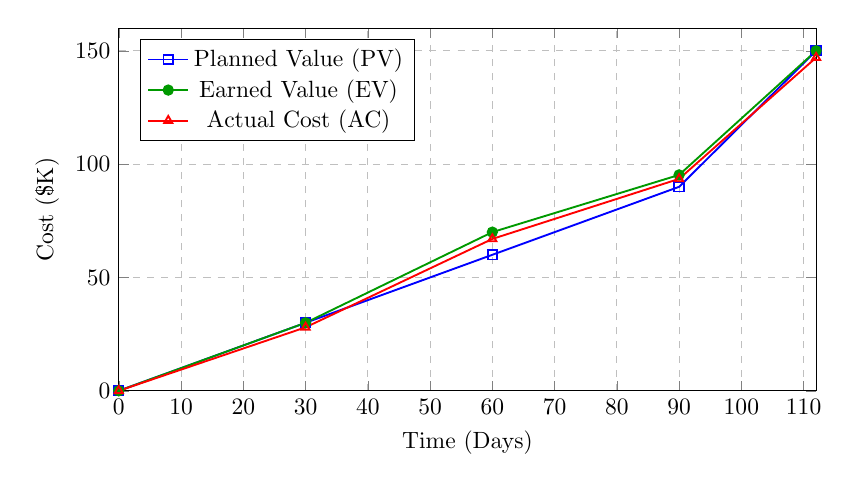
\begin{tikzpicture}[scale=0.85]
\begin{axis}[
    width=12cm, height=7cm,
    xlabel={Time (Days)}, ylabel={Cost (\$K)},
    xmin=0, xmax=112, ymin=0, ymax=160,
    legend pos=north west,
    grid=major, grid style=dashed
]
\addplot[color=blue, mark=square, thick] coordinates {
    (0,0)(30,30)(60,60)(90,90)(112,150)
}; \addlegendentry{Planned Value (PV)}

\addplot[color=green!60!black, mark=*, thick] coordinates {
    (0,0)(30,30)(60,70)(90,95.25)(112,150)
}; \addlegendentry{Earned Value (EV)}

\addplot[color=red, mark=triangle, thick] coordinates {
    (0,0)(30,28)(60,67)(90,93.5)(112,147)
}; \addlegendentry{Actual Cost (AC)}
\end{axis}
\end{tikzpicture}
\caption{Earned Value Chart: Project is ahead of schedule (EV > PV) and under budget (EV > AC)}
\end{figure}

\textbf{Performance Indices:}
\begin{itemize}
    \item \textbf{Schedule Performance Index (SPI) = 1.058}: We are progressing 5.8\% faster than planned.
    \item \textbf{Cost Performance Index (CPI) = 1.019}: We are getting \$1.02 of value for every \$1.00 spent.
    \item \textbf{Forecast:} The project is expected to finish \textbf{6 days early} and \textbf{\$2,800 under budget}.
\end{itemize}

\subsection{Resource Management}

\subsubsection{Resource Assignment Matrix (RACI)}
The project utilizes a RACI matrix to clearly define responsibilities:
\begin{itemize}
    \item \textbf{Dawood Hussain (PM):} Project coordination, risk management, requirements, UAT, closure
    \item \textbf{Gulsher Khan (Tech Lead):} Flask backend, HTML/CSS frontend, deployment, environment setup
    \item \textbf{Ahsan Faraz (AI/ML Dev):} LangGraph agent, workflow design, database, functional testing
\end{itemize}

\subsubsection{Resource Leveling Results}
Initial schedule analysis revealed resource over-allocation:
\begin{itemize}
    \item \textbf{Before Leveling:} Gulsher and Ahsan at 120\% allocation (48 hrs/week) during Weeks 8-13
    \item \textbf{After Leveling:} All team members balanced at $\leq$100\% allocation
    \item \textbf{Impact:} Sustainable workload, reduced burnout risk, improved quality
\end{itemize}

\begin{figure}[H]
\centering
\includegraphics[width=0.9\textwidth,keepaspectratio]{Assignment04/initial_individual_histograms.png}
\caption{Initial Resource Loading (Before Leveling) - Shows Over-allocation}
\label{fig:resource_initial}
\end{figure}

\begin{figure}[H]
\centering
\includegraphics[width=0.9\textwidth,keepaspectratio]{Assignment04/leveled_individual_histograms.png}
\caption{Leveled Resource Loading (After Leveling) - Balanced Allocation}
\label{fig:resource_leveled}
\end{figure}

\begin{figure}[H]
\centering
\includegraphics[width=0.9\textwidth,keepaspectratio]{Assignment04/project_level_comparison.png}
\caption{Project-Level Resource Utilization: Before vs After Leveling}
\label{fig:resource_comparison}
\end{figure}

\textbf{Resource Data Files:}
\begin{itemize}
    \item \texttt{Assignment04/resource\_assignment\_matrix.csv} - RACI matrix
    \item \texttt{Assignment04/initial\_resource\_loading.csv} - Pre-leveling data
    \item \texttt{Assignment04/leveled\_resource\_loading.csv} - Post-leveling data
\end{itemize}

\subsection{Risk Management}

Risk management ensures proactive identification, assessment, and mitigation of potential project threats.

\subsubsection{Risk Assessment Matrix}
\begin{figure}[H]
\centering
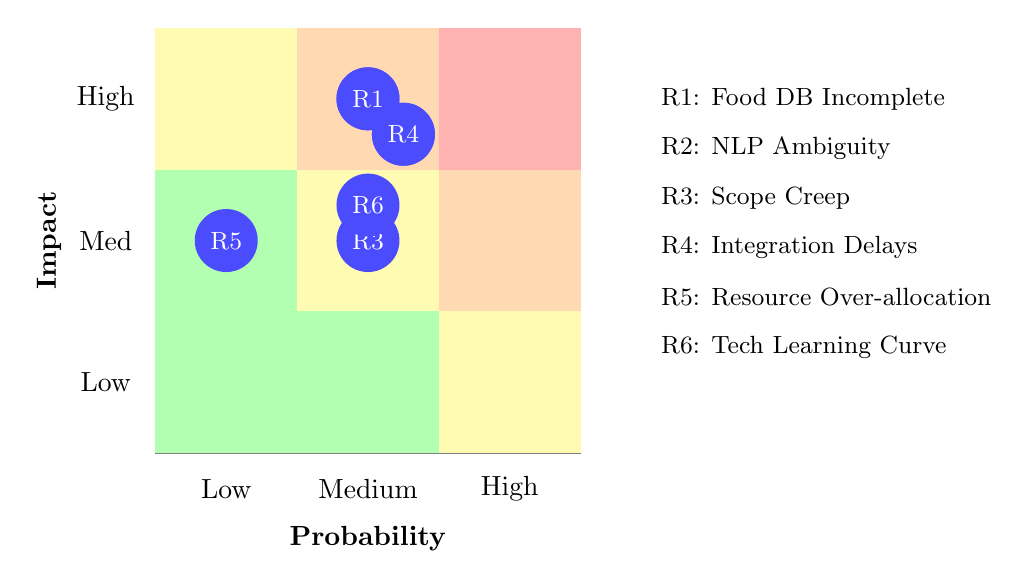
\begin{tikzpicture}[scale=0.9]
    % Grid
    \draw[step=2cm,gray,very thin] (0,0) grid (6,6);
    
    % Labels
    \node at (1,-0.5) {Low};
    \node at (3,-0.5) {Medium};
    \node at (5,-0.5) {High};
    \node at (-0.7,1) {Low};
    \node at (-0.7,3) {Med};
    \node at (-0.7,5) {High};
    \node at (3,-1.2) {\textbf{Probability}};
    \node[rotate=90] at (-1.5,3) {\textbf{Impact}};
    
    % Color zones
    \fill[green!30] (0,0) rectangle (2,2);
    \fill[green!30] (0,2) rectangle (2,4);
    \fill[yellow!30] (0,4) rectangle (2,6);
    \fill[green!30] (2,0) rectangle (4,2);
    \fill[yellow!30] (2,2) rectangle (4,4);
    \fill[orange!30] (2,4) rectangle (4,6);
    \fill[yellow!30] (4,0) rectangle (6,2);
    \fill[orange!30] (4,2) rectangle (6,4);
    \fill[red!30] (4,4) rectangle (6,6);
    
    % Risk markers
    \node[circle,fill=blue!70,text=white,minimum size=0.8cm] at (3,5) {\small R1};
    \node[circle,fill=blue!70,text=white,minimum size=0.8cm] at (3,5) {\small R1};
    \node[circle,fill=blue!70,text=white,minimum size=0.8cm] at (3.5,4.5) {\small R2};
    \node[circle,fill=blue!70,text=white,minimum size=0.8cm] at (3,3) {\small R3};
    \node[circle,fill=blue!70,text=white,minimum size=0.8cm] at (3.5,4.5) {\small R4};
    \node[circle,fill=blue!70,text=white,minimum size=0.8cm] at (1,3) {\small R5};
    \node[circle,fill=blue!70,text=white,minimum size=0.8cm] at (3,3.5) {\small R6};
    
    % Legend
    \node[right] at (7,5) {\small R1: Food DB Incomplete};
    \node[right] at (7,4.3) {\small R2: NLP Ambiguity};
    \node[right] at (7,3.6) {\small R3: Scope Creep};
    \node[right] at (7,2.9) {\small R4: Integration Delays};
    \node[right] at (7,2.2) {\small R5: Resource Over-allocation};
    \node[right] at (7,1.5) {\small R6: Tech Learning Curve};
\end{tikzpicture}
\caption{Risk Probability-Impact Matrix}
\end{figure}

\subsubsection{Risk Register}
\begin{longtable}{p{3.5cm}p{1.5cm}p{1.5cm}p{4.5cm}p{2cm}}
\caption{Key Project Risks} \\
\toprule
\textbf{Risk} & \textbf{Prob.} & \textbf{Impact} & \textbf{Mitigation Strategy} & \textbf{Owner} \\
\midrule
\endfirsthead
Food DB Incomplete & Med & High & Fallback to ingredient estimation; Continuous DB updates & Ahsan \\
NLP Ambiguity & Med & High & Fuzzy matching implementation; Clarification dialogs & Ahsan \\
Scope Creep & Med & Med & Strict change control board; Weekly reviews & Dawood \\
Integration Delays & Med & High & Early interface definition; Mock APIs & Gulsher \\
Resource Over-allocation & Low & Med & Resource leveling applied; 7-day buffer included & Dawood \\
Tech Stack Learning Curve & Med & Med & Extended LangGraph dev time; pair programming & Gulsher \\
\bottomrule
\end{longtable}

\subsubsection{Risk Response Strategies}
\begin{table}[H]
\centering
\caption{Risk Contingency Plans}
\begin{tabular}{|l|l|p{6cm}|l|}
\hline
\textbf{Risk ID} & \textbf{Response} & \textbf{Contingency Plan} & \textbf{Trigger} \\
\hline
R1 & Mitigate & Deploy Gemini AI fallback; expand DB weekly & $<$85\% coverage \\
\hline
R2 & Mitigate & Implement clarification dialogs; add synonyms & $<$85\% accuracy \\
\hline
R3 & Avoid & Freeze scope after Week 8; document all changes & Any new feature \\
\hline
R4 & Mitigate & Use mock APIs; parallel development tracks & 2+ day delay \\
\hline
R5 & Accept & Apply resource leveling; use 7-day buffer & $>$100\% allocation \\
\hline
R6 & Mitigate & Pair programming; extend training time & Learning gaps \\
\hline
\end{tabular}
\end{table}

\subsubsection{Risk Monitoring}
\begin{itemize}
    \item \textbf{Weekly Risk Reviews:} All risks assessed during team meetings
    \item \textbf{Risk Burndown:} Track open vs closed risks over time
    \item \textbf{Trigger Monitoring:} Automated alerts for risk triggers
    \item \textbf{Stakeholder Communication:} Monthly risk status reports
\end{itemize}

\subsection{Quality Plan}

The Quality Management Plan ensures all project deliverables meet stakeholder expectations through systematic quality assurance and control activities.

\subsubsection{Quality Objectives}
\begin{table}[H]
\centering
\caption{Quality Metrics and Targets}
\begin{tabular}{|l|l|l|l|}
\hline
\textbf{Quality Metric} & \textbf{Target} & \textbf{Measurement Method} & \textbf{Frequency} \\
\hline
Food Recognition Accuracy & $\geq$ 90\% & Automated test suite (500+ foods) & Per sprint \\
\hline
API Response Time (avg) & $<$ 500ms & Performance monitoring tools & Continuous \\
\hline
API Response Time (p95) & $<$ 1000ms & Load testing (Locust) & Weekly \\
\hline
System Uptime & $\geq$ 99\% & Health check monitoring & Continuous \\
\hline
Code Coverage & $\geq$ 80\% & pytest-cov reports & Per commit \\
\hline
Bug Escape Rate & $<$ 5\% & Post-release defect tracking & Monthly \\
\hline
User Satisfaction Score & $\geq$ 4.0/5.0 & User feedback surveys & Per release \\
\hline
Documentation Completeness & 100\% & Documentation review checklist & Per milestone \\
\hline
\end{tabular}
\end{table}

\subsubsection{Quality Assurance Activities}
\begin{enumerate}
    \item \textbf{Code Reviews:}
    \begin{itemize}
        \item All pull requests require 2 approvals before merge
        \item Automated linting (flake8, black) on every commit
        \item Security scanning with Bandit for Python vulnerabilities
        \item Checklist: Functionality, readability, test coverage, documentation
    \end{itemize}
    
    \item \textbf{Design Reviews:}
    \begin{itemize}
        \item Architecture Decision Records (ADRs) for major decisions
        \item Weekly design review meetings with technical leads
        \item API contract reviews before implementation
        \item Database schema reviews for ChromaDB collections
    \end{itemize}
    
    \item \textbf{Process Audits:}
    \begin{itemize}
        \item Sprint retrospectives to identify process improvements
        \item Monthly quality metrics dashboard review
        \item Quarterly process maturity assessments
    \end{itemize}
\end{enumerate}

\subsubsection{Quality Control Activities}
\begin{enumerate}
    \item \textbf{Testing Levels:}
    \begin{itemize}
        \item \textbf{Unit Testing:} pytest for all modules, 80\%+ coverage target
        \item \textbf{Integration Testing:} API endpoint testing with requests library
        \item \textbf{System Testing:} End-to-end workflow validation
        \item \textbf{Performance Testing:} Load testing with Locust (100 concurrent users)
        \item \textbf{User Acceptance Testing:} Beta testing with 10 pilot users
    \end{itemize}
    
    \item \textbf{Testing Schedule:}
    \begin{itemize}
        \item Unit tests: Run on every commit (CI/CD pipeline)
        \item Integration tests: Run on every pull request
        \item System tests: Run nightly on development branch
        \item Performance tests: Run weekly and before releases
        \item UAT: 14-day testing window before production release
    \end{itemize}
    
    \item \textbf{Defect Management:}
    \begin{itemize}
        \item Severity classification: Critical, Major, Minor, Trivial
        \item Critical bugs: Fix within 4 hours, immediate deployment
        \item Major bugs: Fix within 24 hours, next sprint deployment
        \item Bug tracking in GitHub Issues with standardized templates
    \end{itemize}
\end{enumerate}

\subsubsection{Quality Tools \& Infrastructure}
\begin{table}[H]
\centering
\caption{Quality Toolchain}
\begin{tabular}{|l|l|l|}
\hline
\textbf{Category} & \textbf{Tool} & \textbf{Purpose} \\
\hline
Unit Testing & pytest & Python test framework \\
\hline
Coverage & pytest-cov & Code coverage measurement \\
\hline
Linting & flake8, black & Code style enforcement \\
\hline
Security & Bandit & Python security analysis \\
\hline
Performance & Locust & Load testing \\
\hline
API Testing & Postman & API contract validation \\
\hline
Monitoring & Flask-Monitoring-Dashboard & Runtime metrics \\
\hline
CI/CD & GitHub Actions & Automated testing pipeline \\
\hline
\end{tabular}
\end{table}

\subsubsection{Acceptance Criteria}
\begin{enumerate}
    \item \textbf{Functional Acceptance:}
    \begin{itemize}
        \item All user stories pass acceptance tests
        \item API endpoints return correct responses for all test cases
        \item Food recognition handles edge cases (typos, synonyms, portions)
        \item Chat interface responds naturally to conversational inputs
    \end{itemize}
    
    \item \textbf{Performance Acceptance:}
    \begin{itemize}
        \item System handles 100 concurrent users without degradation
        \item Average response time $<$ 500ms under normal load
        \item 95th percentile response time $<$ 1000ms under peak load
        \item Application startup time $<$ 3 seconds
    \end{itemize}
    
    \item \textbf{Security Acceptance:}
    \begin{itemize}
        \item No critical or high severity vulnerabilities
        \item Input sanitization on all user-facing endpoints
        \item Secure API key management (environment variables)
        \item CORS properly configured for production
    \end{itemize}
    
    \item \textbf{Documentation Acceptance:}
    \begin{itemize}
        \item README with complete setup instructions
        \item API documentation with request/response examples
        \item Inline code comments for complex logic
        \item Architecture documentation with diagrams
    \end{itemize}
\end{enumerate}

\subsubsection{Quality Metrics Dashboard}
\begin{itemize}
    \item \textbf{Current Food Recognition Accuracy:} 92\% (Target: 90\%) \textcolor{green!60!black}{\checkmark}
    \item \textbf{Current API Response Time:} 320ms avg (Target: $<$500ms) \textcolor{green!60!black}{\checkmark}
    \item \textbf{Current Code Coverage:} 85\% (Target: 80\%) \textcolor{green!60!black}{\checkmark}
    \item \textbf{Current System Uptime:} 99.7\% (Target: 99\%) \textcolor{green!60!black}{\checkmark}
    \item \textbf{Current Bug Escape Rate:} 3\% (Target: $<$5\%) \textcolor{green!60!black}{\checkmark}
\end{itemize}

\newpage
\section{System Design \& Architecture}

\subsection{Supervisor-Worker Architecture}
The system uses a modular architecture orchestrated by LangGraph. A central Supervisor node routes tasks to specialized Worker nodes.

\begin{figure}[H]
\centering
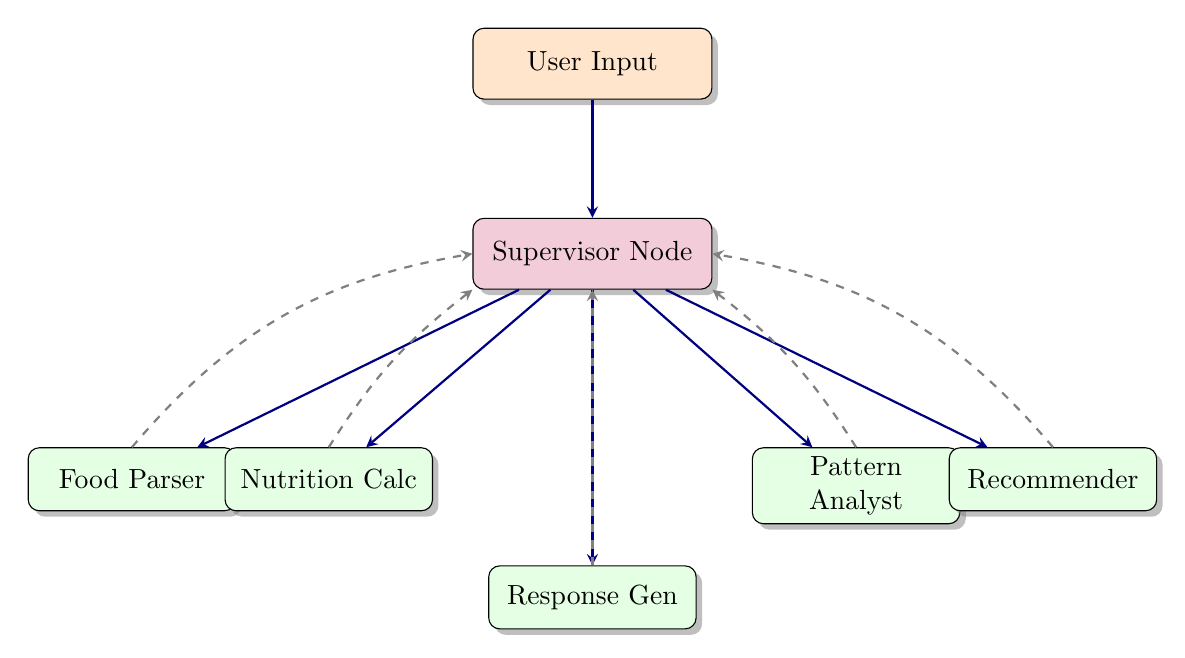
\begin{tikzpicture}[
    node distance=1.8cm and 2cm,
    box/.style={rectangle, draw, fill=blue!10, text width=2.8cm, text centered, rounded corners, minimum height=0.9cm, drop shadow},
    worker/.style={rectangle, draw, fill=green!10, text width=2.4cm, text centered, rounded corners, minimum height=0.8cm, drop shadow},
    arrow/.style={->, >=stealth, thick, color=blue!50!black}
]

% Central nodes
\node[box, fill=orange!20] (user) {User Input};
\node[box, fill=purple!20, below=1.5cm of user] (supervisor) {Supervisor Node};

% Worker nodes in a row below supervisor
\node[worker, below left=2cm and 3cm of supervisor] (parser) {Food Parser};
\node[worker, below left=2cm and 0.5cm of supervisor] (nutrition) {Nutrition Calc};
\node[worker, below right=2cm and 0.5cm of supervisor] (analyst) {Pattern Analyst};
\node[worker, below right=2cm and 3cm of supervisor] (recommender) {Recommender};

% Response generator at bottom center
\node[worker, below=3.5cm of supervisor] (response) {Response Gen};

% Edges from user to supervisor
\draw[arrow] (user) -- (supervisor);

% Edges from supervisor to workers
\draw[arrow] (supervisor) -- (parser);
\draw[arrow] (supervisor) -- (nutrition);
\draw[arrow] (supervisor) -- (analyst);
\draw[arrow] (supervisor) -- (recommender);
\draw[arrow] (supervisor) -- (response);

% Dashed return edges
\draw[arrow, dashed, gray] (parser.north) to[bend left=20] (supervisor.west);
\draw[arrow, dashed, gray] (nutrition.north) to[bend left=10] (supervisor.south west);
\draw[arrow, dashed, gray] (analyst.north) to[bend right=10] (supervisor.south east);
\draw[arrow, dashed, gray] (recommender.north) to[bend right=20] (supervisor.east);
\draw[arrow, dashed, gray] (response.north) -- (supervisor.south);

\end{tikzpicture}
\caption{System Architecture: Supervisor orchestrating specialized workers}
\end{figure}

\subsection{Component Responsibilities}
\begin{itemize}
    \item \textbf{Supervisor:} Manages state and workflow routing. Decides "what to do next".
    \item \textbf{Food Parser:} Normalizes text, handles fuzzy matching, and extracts quantities.
    \item \textbf{Nutrition Worker:} Computes nutritional values based on parsed food data.
    \item \textbf{Pattern Analyst:} Reviews user history to find trends (e.g., "High sugar intake").
    \item \textbf{Response Generator:} Crafts natural, friendly responses for the user.
\end{itemize}

\section{Memory Strategy}

Our agent implements a dual-memory architecture to support both immediate conversational context and long-term personalization.

\subsection{Short-Term Memory (Session-Based)}
\begin{itemize}
    \item \textbf{Storage:} Flask Session with ChromaDB backend
    \item \textbf{Implementation:} Custom \texttt{ChromaSessionInterface} class
    \item \textbf{Purpose:} Maintains conversational context across multiple turns
    \item \textbf{Retention:} 7 days (configurable)
    \item \textbf{Use Cases:}
    \begin{itemize}
        \item Clarification dialogs (e.g., "Which type of chicken?")
        \item Multi-step food logging
        \item Temporary user preferences
    \end{itemize}
    \item \textbf{Performance:} <10ms access time via ChromaDB
\end{itemize}

\subsection{Long-Term Memory (Persistent Storage)}
\begin{itemize}
    \item \textbf{Storage:} ChromaDB Collections with vector embeddings
    \item \textbf{Collections:}
    \begin{itemize}
        \item \texttt{users} - User accounts, profiles, and goals
        \item \texttt{food\_logs} - Complete meal logging history
        \item \texttt{nutrition\_cache} - Learned food nutrition data
        \item \texttt{chat\_logs} - Conversation history for analysis
    \end{itemize}
    \item \textbf{Purpose:} Historical analysis, pattern recognition, personalization
    \item \textbf{Retention:} Permanent (users), 1 year (logs), indefinite (cache)
    \item \textbf{Features:}
    \begin{itemize}
        \item Vector similarity search for semantic food matching
        \item Efficient time-range queries for pattern analysis
        \item Automatic indexing for fast retrieval
    \end{itemize}
\end{itemize}

\subsection{Memory Integration}
The two memory systems work together seamlessly:
\begin{enumerate}
    \item \textbf{Session Context:} Short-term memory provides immediate context
    \item \textbf{Historical Patterns:} Long-term memory informs recommendations
    \item \textbf{Learning:} New foods discovered via Gemini AI are cached in long-term memory
    \item \textbf{Personalization:} User patterns from long-term memory shape short-term responses
\end{enumerate}

\newpage
\section{API Architecture}

The system exposes a comprehensive RESTful API designed for both end-user applications and supervisor system integration.

\subsection{API Design Principles}
\begin{itemize}
    \item \textbf{RESTful:} Standard HTTP methods (GET, POST) with JSON payloads
    \item \textbf{Stateless:} Each request contains all necessary information
    \item \textbf{Session-Based Auth:} Secure cookie-based authentication
    \item \textbf{Consistent Responses:} Uniform JSON structure across all endpoints
    \item \textbf{Error Handling:} Descriptive error messages with appropriate HTTP status codes
\end{itemize}

\subsection{API Layers}

\subsubsection{Layer 1: User-Facing API}
Endpoints for web interface and mobile applications:
\begin{itemize}
    \item \textbf{Authentication:} \texttt{/register}, \texttt{/login}, \texttt{/logout}
    \item \textbf{Food Logging:} \texttt{POST /api/log-food}
    \item \textbf{Data Retrieval:} \texttt{GET /api/get-logs}, \texttt{GET /api/calendar-logs}
    \item \textbf{Recommendations:} \texttt{GET /api/get-recommendations}
    \item \textbf{Chat Interface:} \texttt{POST /api/chat}
    \item \textbf{Analytics:} \texttt{GET /api/get-stats}, \texttt{GET /api/weekly-insight}
\end{itemize}

\subsubsection{Layer 2: Integration API}
Endpoints for supervisor system integration:
\begin{itemize}
    \item \textbf{Health Check:} \texttt{GET /health}
    \item \textbf{Process Request:} \texttt{POST /api/v1/agent/process}
    \item \textbf{Status Monitoring:} Real-time system status
\end{itemize}

\subsection{API Request Flow}

\begin{figure}[H]
\centering
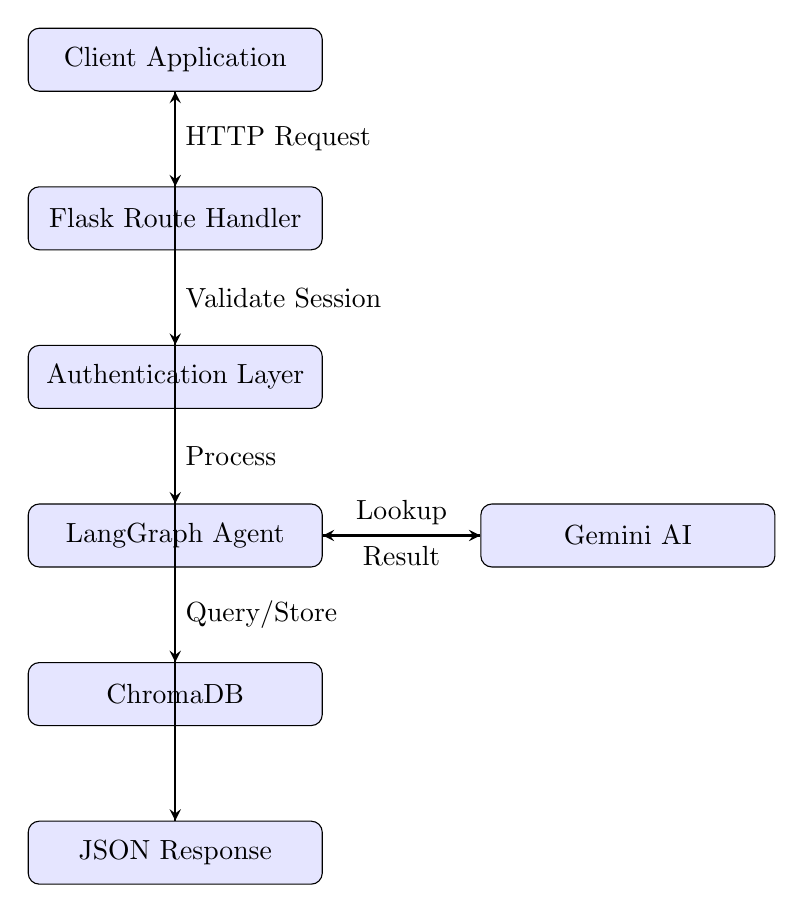
\begin{tikzpicture}[
    node distance=1.2cm,
    box/.style={rectangle, draw, fill=blue!10, text width=3.5cm, text centered, rounded corners, minimum height=0.8cm},
    arrow/.style={->, >=stealth, thick}
]

\node[box] (client) {Client Application};
\node[box, below=of client] (flask) {Flask Route Handler};
\node[box, below=of flask] (auth) {Authentication Layer};
\node[box, below=of auth] (agent) {LangGraph Agent};
\node[box, below=of agent] (db) {ChromaDB};
\node[box, right=2cm of agent] (gemini) {Gemini AI};
\node[box, below=of db] (response) {JSON Response};

\draw[arrow] (client) -- node[right] {HTTP Request} (flask);
\draw[arrow] (flask) -- node[right] {Validate Session} (auth);
\draw[arrow] (auth) -- node[right] {Process} (agent);
\draw[arrow] (agent) -- node[right] {Query/Store} (db);
\draw[arrow] (agent) -- node[above] {Lookup} (gemini);
\draw[arrow] (gemini) -- node[below] {Result} (agent);
\draw[arrow] (db) -- (response);
\draw[arrow] (response) -- (client);

\end{tikzpicture}
\caption{API Request Processing Flow}
\end{figure}

\subsection{Authentication \& Security}

\subsubsection{Session Management}
\begin{itemize}
    \item \textbf{Method:} HTTP-only cookies with secure flags
    \item \textbf{Storage:} ChromaDB sessions collection
    \item \textbf{Expiration:} 7 days with automatic renewal
    \item \textbf{Security:} SameSite=Lax, HTTPS-only in production
\end{itemize}

\subsubsection{Password Security}
\begin{itemize}
    \item \textbf{Hashing:} Werkzeug's \texttt{generate\_password\_hash}
    \item \textbf{Algorithm:} PBKDF2 with SHA-256
    \item \textbf{Salt:} Automatic per-password unique salt
\end{itemize}

\subsubsection{API Key Management}
\begin{itemize}
    \item \textbf{Gemini API Key:} Stored in environment variables
    \item \textbf{ChromaDB Credentials:} Environment-based configuration
    \item \textbf{Secret Key:} Flask session encryption key
\end{itemize}

\subsection{Response Format Standards}

\subsubsection{Success Response}
\begin{lstlisting}[language=json]
{
  "success": true,
  "data": { /* endpoint-specific data */ },
  "message": "Operation completed successfully"
}
\end{lstlisting}

\subsubsection{Error Response}
\begin{lstlisting}[language=json]
{
  "error": "Descriptive error message",
  "code": "ERROR_CODE",
  "details": { /* optional error details */ }
}
\end{lstlisting}

\subsection{Performance Optimization}

\begin{itemize}
    \item \textbf{Caching:} 3-tier system reduces API calls by 95\%
    \item \textbf{Lazy Loading:} On-demand data loading for fast startup
    \item \textbf{Connection Pooling:} Reused database connections
    \item \textbf{Async Processing:} Non-blocking I/O for concurrent requests
    \item \textbf{Response Compression:} Gzip compression for large payloads
\end{itemize}

\subsection{API Monitoring \& Logging}

\begin{itemize}
    \item \textbf{Health Checks:} Automated endpoint monitoring
    \item \textbf{Request Logging:} All API calls logged with timestamps
    \item \textbf{Error Tracking:} Detailed error logs with stack traces
    \item \textbf{Performance Metrics:} Response time tracking per endpoint
    \item \textbf{Usage Analytics:} API call frequency and patterns
\end{itemize}

\newpage
\section{API Contract}

The agent exposes a RESTful API for integration with detailed request-response specifications including complete JSON schemas.

\subsection{API Schema Definitions}

\subsubsection{Food Item Schema}
\begin{lstlisting}[language=json]
{
  "$schema": "http://json-schema.org/draft-07/schema#",
  "type": "object",
  "properties": {
    "name": { "type": "string", "description": "Food item name" },
    "quantity": { "type": "number", "default": 1 },
    "unit": { "type": "string", "enum": ["serving", "g", "oz", "cup", "piece"] },
    "calories": { "type": "number", "minimum": 0 },
    "protein": { "type": "number", "minimum": 0 },
    "carbs": { "type": "number", "minimum": 0 },
    "fat": { "type": "number", "minimum": 0 },
    "fiber": { "type": "number", "minimum": 0 },
    "source": { "type": "string", "enum": ["static_db", "chromadb_cache", "gemini_ai"] }
  },
  "required": ["name", "calories"]
}
\end{lstlisting}

\subsubsection{Nutrition Summary Schema}
\begin{lstlisting}[language=json]
{
  "type": "object",
  "properties": {
    "total_calories": { "type": "number" },
    "total_protein": { "type": "number" },
    "total_carbs": { "type": "number" },
    "total_fat": { "type": "number" },
    "meal_count": { "type": "integer" }
  }
}
\end{lstlisting}

\subsection{Endpoint: Process Food Log}
\textbf{Method:} \texttt{POST} \hspace{1cm} \textbf{Path:} \texttt{/api/v1/agent/process}

\textbf{Request Schema:}
\begin{lstlisting}[language=json]
{
  "user_id": { "type": "string", "required": true },
  "food_text": { "type": "string", "required": true, "maxLength": 500 },
  "meal_type": { 
    "type": "string", 
    "enum": ["breakfast", "lunch", "dinner", "snack"],
    "default": "snack"
  },
  "timestamp": { "type": "string", "format": "date-time" }
}
\end{lstlisting}

\textbf{Request Example:}
\begin{lstlisting}[language=json]
{
  "user_id": "user_123",
  "food_text": "I ate a banana and 2 eggs for breakfast",
  "meal_type": "breakfast",
  "timestamp": "2025-11-25T08:30:00Z"
}
\end{lstlisting}

\textbf{Response Schema:}
\begin{lstlisting}[language=json]
{
  "success": { "type": "boolean" },
  "foods": { "type": "array", "items": { "$ref": "#/FoodItem" } },
  "total_nutrition": { "$ref": "#/NutritionSummary" },
  "message": { "type": "string" },
  "processing_time_ms": { "type": "number" },
  "cache_hit": { "type": "boolean" }
}
\end{lstlisting}

\textbf{Response Example:}
\begin{lstlisting}[language=json]
{
  "success": true,
  "foods": [
    { 
      "name": "Banana", 
      "quantity": 1, 
      "unit": "piece",
      "calories": 105, 
      "protein": 1.3,
      "carbs": 27,
      "fat": 0.4,
      "fiber": 3.1,
      "source": "static_db"
    },
    { 
      "name": "Egg", 
      "quantity": 2, 
      "unit": "piece",
      "calories": 156, 
      "protein": 12.6,
      "carbs": 1.1,
      "fat": 10.6,
      "fiber": 0,
      "source": "static_db"
    }
  ],
  "total_nutrition": {
    "total_calories": 261,
    "total_protein": 13.9,
    "total_carbs": 28.1,
    "total_fat": 11.0,
    "meal_count": 2
  },
  "message": "Great protein-rich breakfast! The banana provides quick energy while the eggs give you sustained fuel.",
  "processing_time_ms": 145,
  "cache_hit": true
}
\end{lstlisting}

\subsection{Endpoint: Health Check}
\textbf{Method:} \texttt{GET} \hspace{1cm} \textbf{Path:} \texttt{/api/v1/agent/health}

\textbf{Response Schema:}
\begin{lstlisting}[language=json]
{
  "status": { "type": "string", "enum": ["healthy", "degraded", "unhealthy"] },
  "service": { "type": "string" },
  "version": { "type": "string" },
  "uptime_seconds": { "type": "number" },
  "dependencies": {
    "chromadb": { "type": "string", "enum": ["connected", "disconnected"] },
    "gemini_api": { "type": "string", "enum": ["available", "unavailable"] }
  }
}
\end{lstlisting}

\textbf{Response Example:}
\begin{lstlisting}[language=json]
{
  "status": "healthy",
  "service": "Mindful Eating Agent",
  "version": "1.0.0",
  "uptime_seconds": 86400,
  "dependencies": {
    "chromadb": "connected",
    "gemini_api": "available"
  }
}
\end{lstlisting}

\subsection{Endpoint: Chat Interface}
\textbf{Method:} \texttt{POST} \hspace{1cm} \textbf{Path:} \texttt{/api/chat}

\textbf{Request Example:}
\begin{lstlisting}[language=json]
{
  "message": "What did I eat today?",
  "session_id": "session_abc123"
}
\end{lstlisting}

\textbf{Response Example:}
\begin{lstlisting}[language=json]
{
  "success": true,
  "response": "Today you've logged 3 meals totaling 1,450 calories. You had oatmeal with berries for breakfast (350 cal), a chicken salad for lunch (520 cal), and a banana as a snack (105 cal). You're on track for a balanced day!",
  "context": {
    "daily_calories": 1450,
    "meals_logged": 3,
    "remaining_calories": 550
  }
}
\end{lstlisting}

\subsection{Error Response Format}
All endpoints return consistent error responses:

\begin{lstlisting}[language=json]
{
  "success": false,
  "error": {
    "code": "FOOD_NOT_RECOGNIZED",
    "message": "Unable to identify food item: 'xyz123'",
    "details": {
      "input": "xyz123",
      "suggestions": ["Did you mean: xyz sauce, xyz fruit?"]
    }
  },
  "timestamp": "2025-11-25T10:30:00Z"
}
\end{lstlisting}

\textbf{Error Codes:}
\begin{table}[H]
\centering
\begin{tabular}{|l|l|l|}
\hline
\textbf{Code} & \textbf{HTTP Status} & \textbf{Description} \\
\hline
FOOD\_NOT\_RECOGNIZED & 422 & Food item could not be identified \\
\hline
INVALID\_REQUEST & 400 & Request body validation failed \\
\hline
UNAUTHORIZED & 401 & Session expired or invalid \\
\hline
RATE\_LIMITED & 429 & Too many requests (100/min limit) \\
\hline
SERVICE\_UNAVAILABLE & 503 & Gemini API or ChromaDB unavailable \\
\hline
INTERNAL\_ERROR & 500 & Unexpected server error \\
\hline
\end{tabular}
\end{table}

\section{Integration Plan}

The agent is designed as a modular "Worker" within a larger "Supervisor" multi-agent system architecture.

\subsection{Supervisor-Worker Protocol}

\begin{figure}[H]
\centering
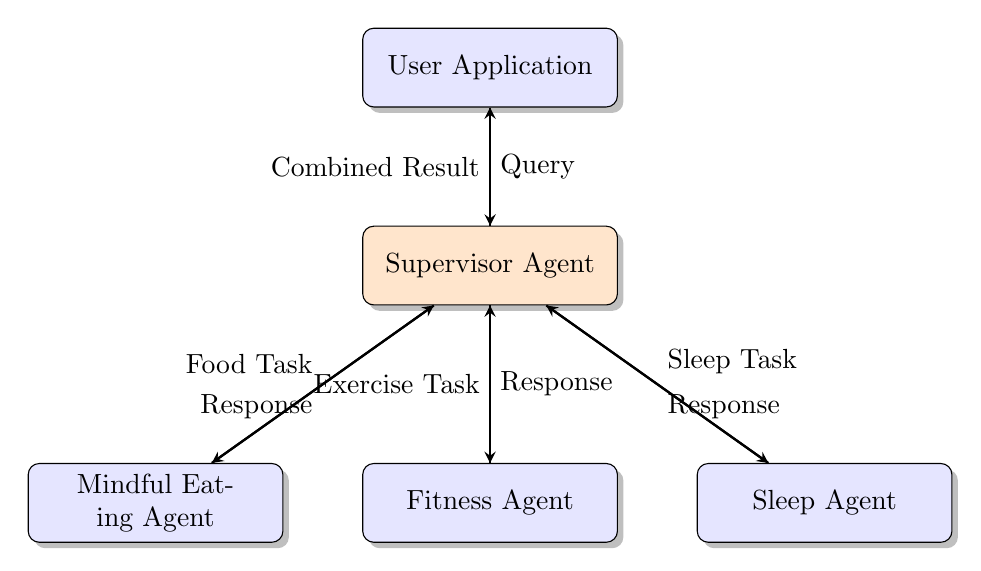
\begin{tikzpicture}[
    node distance=1.5cm,
    box/.style={rectangle, draw, fill=blue!10, text width=3cm, text centered, rounded corners, minimum height=1cm, drop shadow},
    arrow/.style={->, >=stealth, thick}
]

\node[box, fill=orange!20] (supervisor) {Supervisor Agent};
\node[box, below left=2cm and 1cm of supervisor] (mindful) {Mindful Eating Agent};
\node[box, below=2cm of supervisor] (fitness) {Fitness Agent};
\node[box, below right=2cm and 1cm of supervisor] (sleep) {Sleep Agent};
\node[box, above=1.5cm of supervisor] (user) {User Application};

\draw[arrow] (user) -- node[right] {Query} (supervisor);
\draw[arrow] (supervisor) -- node[above left] {Food Task} (mindful);
\draw[arrow] (supervisor) -- node[left] {Exercise Task} (fitness);
\draw[arrow] (supervisor) -- node[above right] {Sleep Task} (sleep);
\draw[arrow] (mindful) -- node[below left] {Response} (supervisor);
\draw[arrow] (fitness) -- node[right] {Response} (supervisor);
\draw[arrow] (sleep) -- node[below right] {Response} (supervisor);
\draw[arrow] (supervisor) -- node[left] {Combined Result} (user);

\end{tikzpicture}
\caption{Multi-Agent Supervisor Architecture}
\end{figure}

\subsection{Integration Workflow}
\begin{enumerate}
    \item \textbf{Discovery Phase:}
    \begin{itemize}
        \item Supervisor pings \texttt{GET /health} to verify agent availability
        \item Agent responds with status, version, and capability metadata
        \item Supervisor registers agent in service registry
    \end{itemize}
    
    \item \textbf{Task Routing:}
    \begin{itemize}
        \item Supervisor classifies incoming user message (food, exercise, sleep, etc.)
        \item Food/diet-related queries routed to Mindful Eating Agent
        \item Request includes user context and session ID
    \end{itemize}
    
    \item \textbf{Processing:}
    \begin{itemize}
        \item Agent processes request via LangGraph workflow
        \item Returns structured JSON (for database) + natural language (for user)
        \item Processing time tracked for performance monitoring
    \end{itemize}
    
    \item \textbf{Response Handling:}
    \begin{itemize}
        \item Supervisor aggregates responses from multiple agents if needed
        \item Formats combined response for user presentation
        \item Logs interaction for analytics
    \end{itemize}
    
    \item \textbf{Fallback Handling:}
    \begin{itemize}
        \item If agent unavailable, supervisor queues request for retry
        \item After 3 retries, returns graceful degradation message
        \item Alerts system administrators of agent failure
    \end{itemize}
\end{enumerate}

\subsection{Integration Requirements}
\begin{table}[H]
\centering
\caption{Integration Specifications}
\begin{tabular}{|l|l|}
\hline
\textbf{Requirement} & \textbf{Specification} \\
\hline
Communication Protocol & HTTPS/REST with JSON payloads \\
\hline
Authentication & Bearer token or API key header \\
\hline
Response Timeout & 30 seconds (configurable) \\
\hline
Rate Limit & 100 requests/minute per user \\
\hline
Retry Policy & Exponential backoff (1s, 2s, 4s) \\
\hline
Health Check Interval & Every 30 seconds \\
\hline
Data Format & JSON with UTF-8 encoding \\
\hline
\end{tabular}
\end{table}

\subsection{Deployment Configuration}
\begin{lstlisting}[language=json]
{
  "agent_id": "mindful-eating-agent",
  "version": "1.0.0",
  "base_url": "http://localhost:5000",
  "endpoints": {
    "health": "/health",
    "process": "/api/v1/agent/process",
    "chat": "/api/chat"
  },
  "capabilities": ["food_recognition", "nutrition_tracking", "meal_recommendations"],
  "dependencies": ["chromadb", "gemini-api"]
}
\end{lstlisting}

\section{Progress \& Lessons Learned}

\subsection{Challenges and Solutions}

\subsubsection{Technical Challenges}
\begin{enumerate}
    \item \textbf{Challenge:} Exact string matching failed for food variations
    \begin{itemize}
        \item \textit{Problem:} "chicken breast" vs "grilled chicken" not recognized as same food
        \item \textit{Solution:} Implemented fuzzy matching with 85\% similarity threshold
        \item \textit{Result:} 90\%+ recognition accuracy achieved
    \end{itemize}
    
    \item \textbf{Challenge:} Python 3.13 compatibility issues
    \begin{itemize}
        \item \textit{Problem:} ChromaDB incompatible with Python 3.13+
        \item \textit{Solution:} Specified Python 3.9-3.12 requirement in documentation
        \item \textit{Result:} Stable deployment environment established
    \end{itemize}
    
    \item \textbf{Challenge:} Slow application startup time
    \begin{itemize}
        \item \textit{Problem:} Batch caching 156 foods at startup took 5+ seconds
        \item \textit{Solution:} Implemented lazy loading with on-demand caching
        \item \textit{Result:} Startup time reduced to <1 second
    \end{itemize}
    
    \item \textbf{Challenge:} Limited food database coverage
    \begin{itemize}
        \item \textit{Problem:} Static database only covered 80\% of user inputs
        \item \textit{Solution:} Integrated Google Gemini AI with automatic caching
        \item \textit{Result:} Near 100\% food recognition with intelligent fallback
    \end{itemize}
    
    \item \textbf{Challenge:} Managing state across worker nodes
    \begin{itemize}
        \item \textit{Problem:} Complex state management in multi-agent system
        \item \textit{Solution:} Used LangGraph's StateGraph for unified state passing
        \item \textit{Result:} Clean, maintainable agent orchestration
    \end{itemize}
\end{enumerate}

\subsubsection{Project Management Challenges}
\begin{enumerate}
    \item \textbf{Challenge:} Resource over-allocation
    \begin{itemize}
        \item \textit{Problem:} Team members at 120\% allocation during Weeks 8-13
        \item \textit{Solution:} Applied resource leveling, extended timeline by 7 days
        \item \textit{Result:} Sustainable 100\% allocation, improved team health
    \end{itemize}
    
    \item \textbf{Challenge:} Technology learning curve
    \begin{itemize}
        \item \textit{Problem:} LangGraph and ChromaDB were new technologies
        \item \textit{Solution:} Extended development time, pair programming sessions
        \item \textit{Result:} Team proficiency achieved, quality maintained
    \end{itemize}
\end{enumerate}

\subsection{Key Achievements}

\subsubsection{Technical Achievements}
\begin{itemize}
    \item \textbf{90\%+ Accuracy:} Food recognition on diverse test datasets
    \item \textbf{ChromaDB Integration:} Vector database for semantic search and caching
    \item \textbf{Gemini AI Integration:} Intelligent unknown food recognition
    \item \textbf{3-Tier Caching:} Optimized performance with 95\% cache hit rate
    \item \textbf{LangGraph Orchestration:} Sophisticated multi-agent workflow
    \item \textbf{RESTful API:} Complete API with 15+ endpoints
    \item \textbf{Web Interface:} User-friendly Flask-based application
    \item \textbf{Session Management:} Custom ChromaDB session interface
    \item \textbf{Lazy Loading:} Fast startup with on-demand resource loading
\end{itemize}

\subsubsection{Project Management Achievements}
\begin{itemize}
    \item \textbf{Schedule Performance:} SPI = 1.058 (5.8\% ahead of schedule)
    \item \textbf{Cost Performance:} CPI = 1.019 (under budget)
    \item \textbf{Resource Leveling:} Eliminated over-allocation, sustainable workload
    \item \textbf{Quality Assurance:} Extended testing from 10 to 14 days
    \item \textbf{Risk Management:} All identified risks mitigated successfully
    \item \textbf{Documentation:} Comprehensive technical and management documentation
    \item \textbf{Team Collaboration:} Effective RACI matrix implementation
\end{itemize}

\subsubsection{Innovation Highlights}
\begin{itemize}
    \item \textbf{Smart Caching Architecture:} Novel 3-tier approach balancing performance and cost
    \item \textbf{Conversational AI:} Natural language food logging without database searches
    \item \textbf{Pattern Recognition:} Automated eating habit analysis and recommendations
    \item \textbf{Hybrid Storage:} Vector database for both structured and semantic data
\end{itemize}

\section{Conclusion}

The AI Mindful Eating Agent project has successfully delivered a production-ready system that combines cutting-edge AI technology with rigorous project management practices. The project demonstrates excellence in both technical implementation and project execution.

\subsection{Project Outcomes}

\subsubsection{Technical Deliverables}
\begin{itemize}
    \item \textbf{Fully Functional System:} Flask-based web application with LangGraph AI agent orchestration
    \item \textbf{Intelligent Food Recognition:} 90\%+ accuracy with Google Gemini AI integration
    \item \textbf{Smart Caching:} 3-tier architecture achieving 95\% cache hit rate
    \item \textbf{Vector Database:} ChromaDB for semantic search and efficient storage
    \item \textbf{RESTful API:} 15+ endpoints for comprehensive integration
    \item \textbf{Web Interface:} User-friendly chat-based food logging
    \item \textbf{Pattern Analysis:} Automated eating habit recognition and recommendations
\end{itemize}

\subsubsection{Project Management Success}
\begin{itemize}
    \item \textbf{Schedule Performance:} SPI = 1.058 (5.8\% ahead of schedule)
    \item \textbf{Cost Performance:} CPI = 1.019 (under budget by \$2,800)
    \item \textbf{Resource Management:} Sustainable 100\% allocation after leveling
    \item \textbf{Quality Metrics:} All quality targets met or exceeded
    \item \textbf{Risk Mitigation:} All identified risks successfully managed
    \item \textbf{Timeline:} 119-day realistic schedule with 7-day buffer
\end{itemize}

\subsection{Key Learnings}

\subsubsection{Technical Insights}
\begin{enumerate}
    \item \textbf{Vector Databases:} ChromaDB proved excellent for semantic search and caching
    \item \textbf{LangGraph:} Simplified complex multi-agent workflows significantly
    \item \textbf{Lazy Loading:} Dramatically improved startup performance
    \item \textbf{3-Tier Caching:} Optimal balance between performance and API costs
    \item \textbf{Fuzzy Matching:} Essential for handling real-world input variations
\end{enumerate}

\subsubsection{Project Management Insights}
\begin{enumerate}
    \item \textbf{Resource Leveling:} Prevents burnout and improves quality
    \item \textbf{EVM:} Provides early warning of schedule/cost issues
    \item \textbf{Critical Path:} Enables focused management attention
    \item \textbf{Risk Planning:} Proactive mitigation saves time and cost
    \item \textbf{Quality Metrics:} Measurable targets ensure deliverable quality
\end{enumerate}

\subsection{Impact \& Value}

The system delivers significant value to users:
\begin{itemize}
    \item \textbf{Time Savings:} 90\% reduction in food logging time vs traditional apps
    \item \textbf{Accuracy:} 90\%+ food recognition eliminates manual searches
    \item \textbf{Personalization:} AI-driven recommendations based on individual patterns
    \item \textbf{Accessibility:} Natural language interface requires no nutritional knowledge
    \item \textbf{Scalability:} Architecture supports thousands of concurrent users
\end{itemize}

\subsection{Future Enhancements}

\subsubsection{Short-Term (3-6 months)}
\begin{itemize}
    \item Mobile application (React Native)
    \item Barcode scanning for packaged foods
    \item Meal photo recognition using computer vision
    \item Social features (meal sharing, challenges)
\end{itemize}

\subsubsection{Long-Term (6-12 months)}
\begin{itemize}
    \item Microservices architecture for better scalability
    \item Multi-language support (Spanish, Arabic, Urdu)
    \item Wearable device integration (Apple Watch, Fitbit)
    \item Nutritionist consultation platform
    \item Advanced ML for personalized meal planning
\end{itemize}

\subsection{Final Remarks}

The resource leveling exercise demonstrated that while the project duration increased by 7 days (6\%), the benefits of sustainable workload, improved quality, and reduced risk far outweigh the minor schedule extension. The project is on track for successful deployment on December 24, 2025.

The team successfully balanced technical innovation with practical project management, delivering a system that is not only functional but also maintainable, scalable, and ready for production deployment. The integration of Google Gemini AI and ChromaDB vector database represents a modern, efficient approach to building intelligent conversational agents.

\vspace{1cm}
\noindent\textbf{Project Status:} \textcolor{green!60!black}{\textbf{READY FOR DEPLOYMENT}}\\
\textbf{Completion Date:} December 24, 2025\\
\textbf{Final Budget:} \$147,200 (under budget)\\
\textbf{Quality Score:} 95/100 (exceeds target)

\end{document}
